\documentclass[tikz]{standalone}

\usetikzlibrary{decorations.pathreplacing} % Pour le bottleneck

\begin{document}
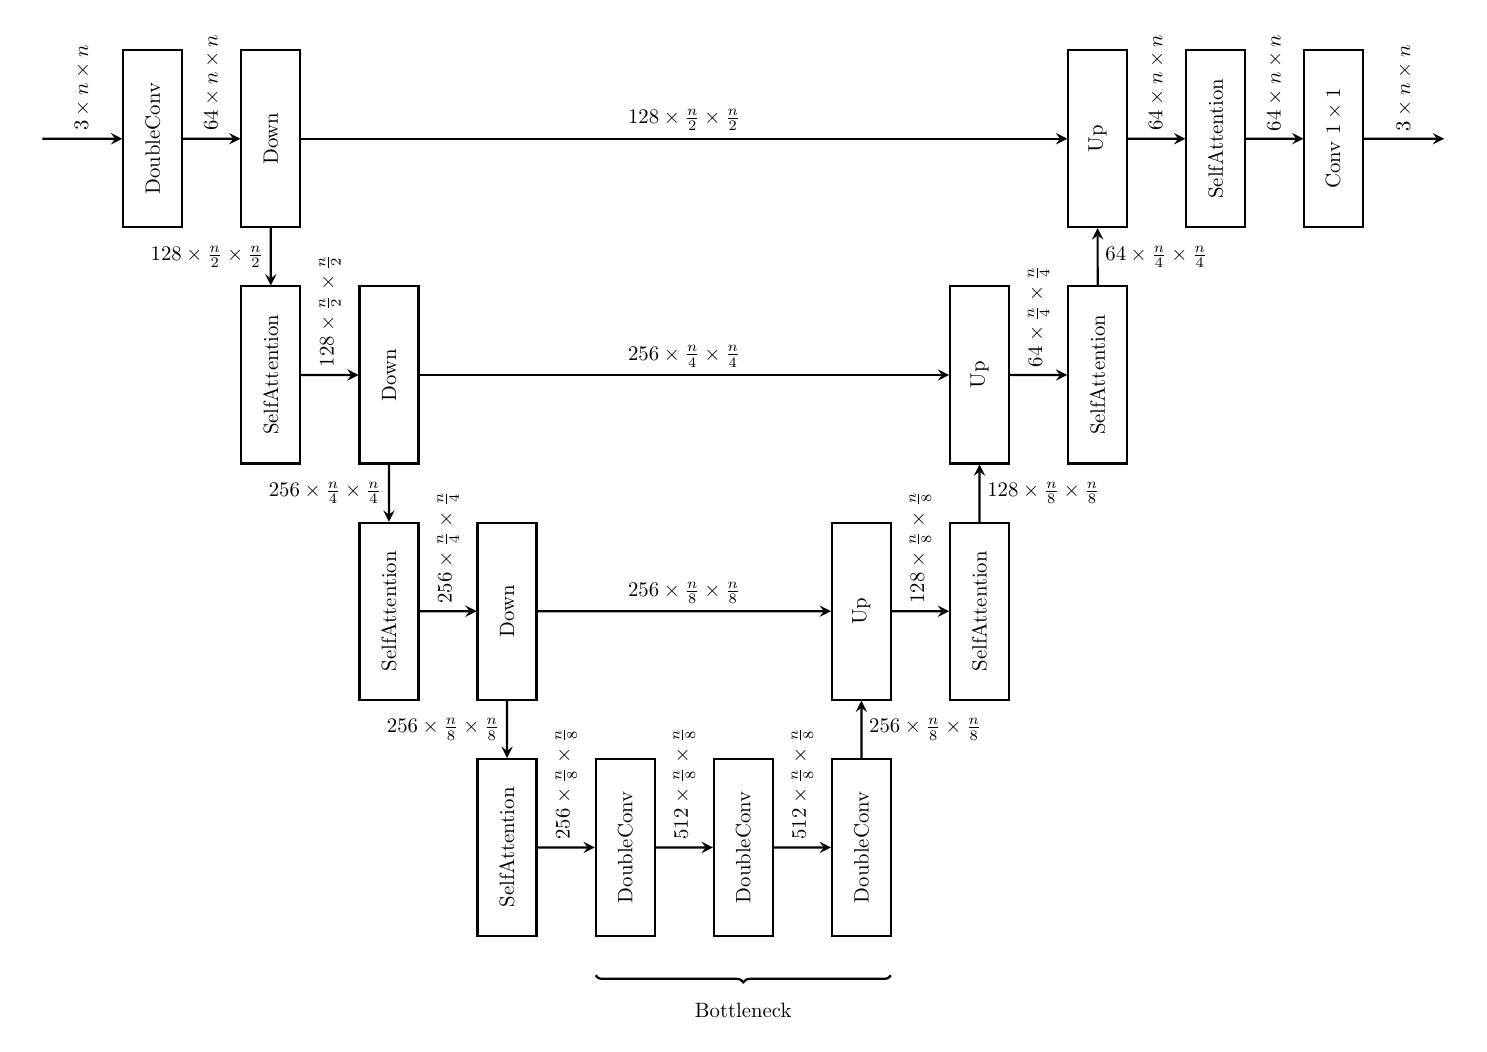
\begin{tikzpicture}[>=stealth, thick, scale=0.75, every node/.style={scale=0.75}, align=center]
    % BLOCKS
    \node (x) at (-2, 0) {};
    \node (inc) at (0, 0) [draw, minimum width=3cm, minimum height=1cm, rotate=90] {DoubleConv};

    \node (down1) at (2, 0) [draw, minimum width=3cm, minimum height=1cm, rotate=90] {Down};
    \node (sa1) at (2, -4) [draw, minimum width=3cm, minimum height=1cm, rotate=90] {SelfAttention};
    \node (down2) at (4, -4) [draw, minimum width=3cm, minimum height=1cm, rotate=90] {Down};
    \node (sa2) at (4, -8) [draw, minimum width=3cm, minimum height=1cm, rotate=90] {SelfAttention};
    \node (down3) at (6, -8) [draw, minimum width=3cm, minimum height=1cm, rotate=90] {Down};
    \node (sa3) at (6, -12) [draw, minimum width=3cm, minimum height=1cm, rotate=90] {SelfAttention};

    \node (bot1) at (8, -12) [draw, minimum width=3cm, minimum height=1cm, rotate=90] {DoubleConv};
    \node (bot2) at (10, -12) [draw, minimum width=3cm, minimum height=1cm, rotate=90] {DoubleConv};
    \node (bot3) at (12, -12) [draw, minimum width=3cm, minimum height=1cm, rotate=90] {DoubleConv};

    \node (up1) at (12, -8) [draw, minimum width=3cm, minimum height=1cm, rotate=90] {Up};
    \node (sa4) at (14, -8) [draw, minimum width=3cm, minimum height=1cm, rotate=90] {SelfAttention};
    \node (up2) at (14, -4) [draw, minimum width=3cm, minimum height=1cm, rotate=90] {Up};
    \node (sa5) at (16, -4) [draw, minimum width=3cm, minimum height=1cm, rotate=90] {SelfAttention};
    \node (up3) at (16, 0) [draw, minimum width=3cm, minimum height=1cm, rotate=90] {Up};
    \node (sa6) at (18, 0) [draw, minimum width=3cm, minimum height=1cm, rotate=90] {SelfAttention};

    \node (outc) at (20, 0) [draw, minimum width=3cm, minimum height=1cm, rotate=90] {Conv $1 \times 1$};
    \node (y) at (22, 0) {};


    % CONNEXIONS WITH DIMENSIONS
    % Direct connexions
    \draw[->] (x) -- node[right, rotate=90] {$3 \times n \times n$} (inc);

    \draw[->] (inc) -- node[right, rotate=90] {$64 \times n \times n$} (down1);
    \draw[->] (down1) -- node[left] {$128 \times \frac{n}{2} \times \frac{n}{2}$} (sa1);
    \draw[->] (sa1) -- node[right, rotate=90] {$128 \times \frac{n}{2} \times \frac{n}{2}$} (down2);
    \draw[->] (down2) -- node[left] {$256 \times \frac{n}{4} \times \frac{n}{4}$} (sa2);
    \draw[->] (sa2) -- node[right, rotate=90] {$256 \times \frac{n}{4} \times \frac{n}{4}$} (down3);
    \draw[->] (down3) -- node[left] {$256 \times \frac{n}{8} \times \frac{n}{8}$} (sa3);

    \draw[->] (sa3) -- node[right, rotate=90] {$256 \times \frac{n}{8} \times \frac{n}{8}$} (bot1);
    \draw[->] (bot1) -- node[right, rotate=90] {$512 \times \frac{n}{8} \times \frac{n}{8}$} (bot2);
    \draw[->] (bot2) -- node[right, rotate=90] {$512 \times \frac{n}{8} \times \frac{n}{8}$} (bot3);
    \draw[->] (bot3) -- node[right] {$256 \times \frac{n}{8} \times \frac{n}{8}$} (up1);

    \draw[->] (up1) -- node[right, rotate=90] {$128 \times \frac{n}{8} \times \frac{n}{8}$} (sa4);
    \draw[->] (sa4) -- node[right] {$128 \times \frac{n}{8} \times \frac{n}{8}$} (up2);
    \draw[->] (up2) -- node[right, rotate=90] {$64 \times \frac{n}{4} \times \frac{n}{4}$} (sa5);
    \draw[->] (sa5) -- node[right] {$64 \times \frac{n}{4} \times \frac{n}{4}$} (up3);
    \draw[->] (up3) -- node[right, rotate=90] {$64 \times n \times n$} (sa6);

    \draw[->] (sa6) -- node[right, rotate=90] {$64 \times n \times n$} (outc);

    \draw[->] (outc) -- node[right, rotate=90] {$3 \times n \times n$} (y);

    % Skip connexions
    \draw[->] (down1) -- node[above] {$128 \times \frac{n}{2} \times \frac{n}{2}$} (up3);
    \draw[->] (down2) -- node[above] {$256 \times \frac{n}{4} \times \frac{n}{4}$} (up2);
    \draw[->] (down3) -- node[above] {$256 \times \frac{n}{8} \times \frac{n}{8}$} (up1);

    % BOTTLENECK CURLY BRACE
    \draw[decoration={brace, mirror, raise=.5cm}, decorate] (7.5, -13.5) -- node[below, yshift=-1cm] {Bottleneck} (12.5, -13.5);
  \end{tikzpicture}
\end{document}